% ============================================================
%  ALDIMI Predict -- Hito 4 (Trabajo Final)
%  Machine Learning 1ACC0057 -- UPC -- 2026-10 -- Grupo 2
% ============================================================
\documentclass[12pt, a4paper]{article}

\usepackage{polyglossia}
\setmainlanguage{spanish}
\usepackage[a4paper, top=2.8cm, bottom=2.8cm, left=3cm, right=3cm]{geometry}
\usepackage{graphicx}
\usepackage{booktabs}
\usepackage{array}
\usepackage{tabularx}
\usepackage{colortbl}
\usepackage[table]{xcolor}
\usepackage{hyperref}
\usepackage{fancyhdr}
\usepackage{titlesec}
\usepackage{enumitem}
\usepackage{float}
\usepackage{caption}
\usepackage{subcaption}
\usepackage{amsmath}
\usepackage{amssymb}
\usepackage{microtype}
\usepackage{parskip}
\usepackage{setspace}
\usepackage{tocloft}
\usepackage{mdframed}
\usepackage{fontspec}
\usepackage{multirow}
\usepackage{makecell}
\usepackage{ragged2e}
\usepackage{needspace}
\PassOptionsToPackage{hyphens}{url}

\setlength{\emergencystretch}{3em}

\setmainfont{DejaVu Serif}
\setsansfont{DejaVu Sans}
\setmonofont{DejaVu Sans Mono}
\renewcommand{\familydefault}{\sfdefault}

% ── Paleta: Esmeralda + Dorado + Granate ──────────────────
\definecolor{primario}{HTML}{0D4B3B}   % verde esmeralda oscuro
\definecolor{secundario}{HTML}{1A936F} % esmeralda medio
\definecolor{dorado}{HTML}{B8860B}     % dorado oscuro
\definecolor{granate}{HTML}{8B1A1A}    % granate (errores/riesgo)
\definecolor{success}{HTML}{2E7D32}    % verde exito
\definecolor{fondoinfo}{HTML}{E8F5E9}  % verde muy claro
\definecolor{fondodest}{HTML}{FFF8E1}  % amarillo muy claro
\definecolor{fondoalerta}{HTML}{FFEBEE}% rojo muy claro
\definecolor{grisc}{HTML}{F5F5F5}      % gris tabla
\definecolor{gristexto}{HTML}{212121}  % casi negro
\definecolor{grismed}{HTML}{546E7A}    % gris medio para captions
\definecolor{azulref}{HTML}{1565C0}    % azul links

% ── Hyperref ─────────────────────────────────────────────
\hypersetup{
  colorlinks = true,
  linkcolor  = primario,
  urlcolor   = azulref,
  citecolor  = primario,
  pdftitle   = {ALDIMI Predict - Trabajo Final},
  pdfauthor  = {Grupo 2 ML 1ACC0057},
}

% ── Cabecera y pie ───────────────────────────────────────
\setlength{\headheight}{28pt}
\pagestyle{fancy}
\fancyhf{}
\fancyhead[L]{%
  \small\color{primario}\textbf{ALDIMI Predict}%
  \color{grismed}\ ---\ Trabajo Final (Hito~4)}
\fancyhead[R]{\small\color{grismed}ML 1ACC0057 \textperiodcentered\ UPC \textperiodcentered\ 2026}
\fancyfoot[C]{\small\color{grismed}\thepage}
\renewcommand{\headrulewidth}{1pt}
\renewcommand{\headrule}{%
  \hbox to\headwidth{\color{primario}\leaders\hrule height\headrulewidth\hfill}}
\renewcommand{\footrulewidth}{0.4pt}
\renewcommand{\footrule}{%
  \hbox to\headwidth{\color{secundario}\leaders\hrule height\footrulewidth\hfill}}

% ── Secciones ────────────────────────────────────────────
\titleformat{\section}
  {\Large\bfseries\color{primario}}{\thesection.}{0.6em}{}
  [\vspace{2pt}\textcolor{secundario}{\rule{\linewidth}{1.2pt}}]
\titleformat{\subsection}
  {\large\bfseries\color{primario}}{\thesubsection.}{0.5em}{}
\titleformat{\subsubsection}
  {\normalsize\bfseries\color{gristexto}}{\thesubsubsection.}{0.4em}{}
\titlespacing{\section}{0pt}{20pt}{8pt}
\titlespacing{\subsection}{0pt}{14pt}{5pt}
\titlespacing{\subsubsection}{0pt}{10pt}{4pt}

% ── Captions ─────────────────────────────────────────────
\captionsetup{
  font={small,color=grismed},
  labelfont={bf,color=primario},
  justification=centering,
  skip=5pt,
}

% ── Columnas personalizadas ───────────────────────────────
\renewcommand{\arraystretch}{1.3}
\newcolumntype{C}[1]{>{\centering\arraybackslash\hspace{0pt}}m{#1}}
\newcolumntype{L}[1]{>{\RaggedRight\arraybackslash\hspace{0pt}}m{#1}}

% ── Cajas ────────────────────────────────────────────────
\newmdenv[
  linecolor=secundario, linewidth=1.2pt,
  backgroundcolor=fondoinfo,
  innerleftmargin=12pt, innerrightmargin=12pt,
  innertopmargin=10pt, innerbottommargin=10pt,
  skipabove=10pt, skipbelow=10pt,
  splitbottomskip=6pt, splittopskip=6pt,
]{infobox}

\newmdenv[
  linecolor=dorado, linewidth=1.5pt,
  backgroundcolor=fondodest,
  innerleftmargin=12pt, innerrightmargin=12pt,
  innertopmargin=10pt, innerbottommargin=10pt,
  skipabove=10pt, skipbelow=10pt,
  splitbottomskip=6pt, splittopskip=6pt,
]{warnbox}

\newmdenv[
  linecolor=success, linewidth=1.5pt,
  backgroundcolor=fondoinfo,
  innerleftmargin=12pt, innerrightmargin=12pt,
  innertopmargin=10pt, innerbottommargin=10pt,
  skipabove=10pt, skipbelow=10pt,
  splitbottomskip=6pt, splittopskip=6pt,
]{successbox}

\newmdenv[
  linecolor=granate, linewidth=1.2pt,
  backgroundcolor=fondoalerta,
  innerleftmargin=12pt, innerrightmargin=12pt,
  innertopmargin=10pt, innerbottommargin=10pt,
  skipabove=10pt, skipbelow=10pt,
  splitbottomskip=6pt, splittopskip=6pt,
]{alertbox}

\graphicspath{{../figures/hito3/}}

% ============================================================
\begin{document}
% ============================================================

% ── PORTADA ─────────────────────────────────────────────
\thispagestyle{empty}
\begin{center}
  \vspace*{1.2cm}
  {\LARGE\bfseries\color{primario} Universidad Peruana de Ciencias Aplicadas}\\[5pt]
  {\large\color{grismed} Facultad de Ingenier\'ia}\\[4pt]
  {\normalsize\color{grismed} MACHINE LEARNING\ ---\ 1ACC0057 \quad|\quad NRC: 3037}

  \vspace{0.8cm}
  \textcolor{primario}{\rule{\linewidth}{2.5pt}}\\[0.5cm]
  {\LARGE\bfseries\color{primario} Trabajo Final\ ---\ Hito~4}\\[0.4cm]
  {\large\bfseries\color{gristexto}
    ALDIMI Predict: Ecosistema Predictivo de\\[3pt]
    Gesti\'on de Recursos y Riesgos}\\[0.5cm]
  \textcolor{primario}{\rule{\linewidth}{2.5pt}}

  \vspace{1cm}
  \begin{tabular}{rl}
    \textbf{Docentes:} & Pinedo Taquia, Jairo \\[3pt]
                       & Zubieta Cardenes, Robert \\[8pt]
    \textbf{Grupo:}    & Grupo 2 \\[6pt]
    \textbf{Fecha:}    & Julio 2026 \\
  \end{tabular}

  \vspace{1.2cm}
  {\large\bfseries\color{primario} Integrantes del equipo}\\[8pt]
  \begin{tabular}{llc}
    \toprule
    \rowcolor{primario!15}
    \textbf{Nombre} & \textbf{C\'odigo} & \textbf{Rol} \\
    \midrule
    {[Integrante 1]} & {[U20XXXXXX]} & Data Scientist \\
    {[Integrante 2]} & {[U20XXXXXX]} & ML Engineer \\
    {[Integrante 3]} & {[U20XXXXXX]} & Data Architect \\
    {[Integrante 4]} & {[U20XXXXXX]} & MLOps / Developer \\
    \bottomrule
  \end{tabular}

  \vspace{1.5cm}
  \textcolor{secundario}{\rule{\linewidth}{0.8pt}}\\[5pt]
  {\small\color{grismed}
    \textbf{ODS alineados:}\quad
    ODS~2 (Hambre Cero)\ \textperiodcentered\
    ODS~3 (Salud y Bienestar)\ \textperiodcentered\
    ODS~10 (Reducci\'on de Desigualdades)
  }
\end{center}
\newpage

% ── INDICE ───────────────────────────────────────────────
\setcounter{page}{1}
\tableofcontents
\newpage

% ============================================================
\section*{Resumen Ejecutivo}
\addcontentsline{toc}{section}{Resumen Ejecutivo}
% ============================================================

El Albergue Divina Misericordia (ALDIMI) atiende gratuitamente a ni\~nos y adolescentes con c\'ancer en situaci\'on de extrema pobreza y se encuentra en plena expansi\'on (\emph{ALDIMI 2.0}): duplicar\'a su capacidad de 50 a 100 familias. Esta expansi\'on es insostenible con procesos manuales: el kardex de almac\'en en hojas de c\'alculo no permite anticipar quiebres de stock, y la priorizaci\'on de la atenci\'on de pacientes depende exclusivamente de la observaci\'on del personal.

\textbf{ALDIMI Predict} aborda ambos problemas con dos frentes de Machine Learning desarrollados bajo la metodolog\'ia CRISP-DM:

\begin{itemize}[leftmargin=1.6em, itemsep=4pt]
  \item \textbf{Frente 1 --- Predicci\'on de inventario:} modelos que anticipan el quiebre de stock de cada art\'iculo a 7 y 14 d\'ias. El modelo seleccionado a 7~d\'ias (XGBoost) alcanza $F_1 = 0{,}9865$ y $\text{AUC} = 0{,}9982$; a 14~d\'ias (Random Forest), $F_1 = 0{,}9721$ y $\text{AUC} = 0{,}9901$.
  \item \textbf{Frente 2 --- Clasificaci\'on de riesgo de pacientes:} un clasificador multiclase (XGBoost) que estima el nivel de prioridad de atenci\'on (Bajo/Medio/Alto) con $F_1\text{-Macro} = 0{,}75$ y $\text{AUC-Macro} = 0{,}9164$ sobre 600 historias sint\'eticas derivadas de las fichas reales de ingreso y reingreso del albergue.
\end{itemize}

Ambos modelos se despliegan en un \emph{dashboard} interactivo (Streamlit) que lee de la \textbf{base de datos com\'un} compartida con el m\'odulo de IA del curso hermano: alertas de stock accionables, evaluaci\'on individual de pacientes con factores de riesgo explicados (valores SHAP) e indicadores globales de gesti\'on. El valor predictivo se traduce en compras y campa\~nas de donaci\'on planificadas con una o dos semanas de anticipaci\'on, y en la priorizaci\'on temprana de pacientes con alta probabilidad de complicaciones, en l\'inea con los ODS~2, 3 y 10.
\newpage

% ============================================================
\section{Contexto del proyecto y entregas previas}
% ============================================================

\subsection{Sobre ALDIMI}

El \textbf{Albergue Divina Misericordia (ALDIMI)} es una organizaci\'on sin fines de lucro que desde 2004 brinda atenci\'on integral y gratuita a ni\~nos y adolescentes con c\'ancer provenientes de las regiones m\'as pobres del Per\'u. La mayor\'ia de los pacientes ---entre 2 y 17 a\~nos--- llegan de la sierra y selva con un diagn\'ostico oncol\'ogico y sin recursos para costearse alojamiento, alimentaci\'on ni acompa\~namiento en Lima mientras reciben tratamiento en los hospitales de referencia.

Con la expansi\'on \textbf{``ALDIMI 2.0''}, el albergue duplicar\'a su capacidad de atenci\'on de 50 a 100 familias simult\'aneas. Este crecimiento hace insostenible la gesti\'on manual de inventario (hojas Excel con errores \texttt{\#REF!}, existencias negativas) y la ausencia de criterios objetivos para priorizar la atenci\'on de pacientes en situaci\'on cr\'itica.

\begin{infobox}
\textbf{Dos problemas cr\'iticos que resuelve el proyecto:}
\begin{enumerate}[leftmargin=1.8em, itemsep=4pt]
  \item \textbf{Gesti\'on de inventario reactiva:} el almac\'en opera sin capacidad de anticipar desabastecimientos. Cuando un art\'iculo se agota, el equipo recurre a compras de emergencia a precios premium o los pacientes quedan sin los insumos necesarios para su dieta oncol\'ogica.
  \item \textbf{Triaje cl\'inico subjetivo:} no existe ning\'un sistema que identifique de forma objetiva qu\'e pacientes presentan mayor riesgo de complicaciones cl\'inicas, por lo que la priorizaci\'on de atenci\'on depende exclusivamente de la experiencia del equipo de salud, que atiende hasta 100 casos simult\'aneos.
\end{enumerate}
\end{infobox}

\subsection{Hito 1 --- Comprensi\'on del negocio y los datos (Semana 5)}

El Hito~1 estableci\'o las bases anal\'iticas del proyecto. Se realizaron las \textbf{fases~1 y~2 de CRISP-DM}: comprensi\'on del negocio y comprensi\'on de los datos.

\textbf{Hallazgos clave del EDA:}
\begin{itemize}[leftmargin=1.5em, itemsep=3pt]
  \item El archivo Excel original de ALDIMI (\texttt{ALMAcen\_upc.xlsx}) presentaba 34 errores \texttt{\#REF!}, existencias negativas en 18 art\'iculos y ausencia de metadatos temporales.
  \item Se identificaron \textbf{19 categor\'ias} de art\'iculos, siendo Menestras y Cereales los insumos de mayor volumen y rotaci\'on.
  \item La distribución de riesgo de los 600 registros sint\'eticos de pacientes mostr\'o un balance deliberado: 33\% Bajo, 33\% Medio, 34\% Alto, calibrado con tablas de incidencia real de c\'anceres pedi\'atricos en el Per\'u.
  \item Se definieron las \textbf{variables objetivo}: \texttt{alerta\_7\_dias} y \texttt{alerta\_14\_dias} (clasificaci\'on binaria) para el Frente~1, y \texttt{nivel\_riesgo} (multiclase Bajo/Medio/Alto) para el Frente~2.
  \item Se detect\'o data leakage en el dataset anual: la resta directa de columnas permit\'ia deducir el target sin entrenamiento. Se decidi\'o trabajar con el \textbf{dataset semanal} para el Frente~1.
\end{itemize}

\subsection{Hito 2 --- Preparaci\'on y Baseline (Semana 7)}

El Hito~2 cubri\'o las \textbf{fases~3 y~4 inicial de CRISP-DM}: preparaci\'on de datos y modelado baseline.

\textbf{Preparaci\'on de datos:}
\begin{itemize}[leftmargin=1.5em, itemsep=3pt]
  \item \textbf{Frente~1 (Inventario):} Label Encoding para categor\'ia (19 valores), \texttt{MinMaxScaler} sobre 7 variables, generaci\'on de \texttt{alerta\_14\_dias} mediante desplazamiento temporal (\textit{shift} $-2$ por art\'iculo). Split 70/30 estratificado.
  \item \textbf{Frente~2 (Pacientes):} Label Encoding ordinal (etapa del c\'ancer, estado f\'isico, nutricional, adherencia, apoyo familiar, acceso a medicamentos, estado emocional, instrucci\'on del cuidador), One-Hot Encoding para 6 variables nominales (sexo, diagn\'ostico, tipo de tratamiento, motivo de ingreso/reingreso, lugar de procedencia). \texttt{MinMaxScaler} sobre variables num\'ericas continuas.
\end{itemize}

\textbf{Resultados baseline:} Se entrenaron tres modelos para cada frente (\'Arbol de Decisi\'on, Naive Bayes y KNN) con hiperpar\'ametros iniciales. Los resultados en el conjunto de prueba fueron:

\begin{center}
\begin{tabular}{lcccc}
  \toprule
  \rowcolor{primario!90}
  \textcolor{white}{\textbf{Frente}} &
  \textcolor{white}{\textbf{Mejor modelo}} &
  \textcolor{white}{\textbf{$F_1$ / $F_1$-Mac.}} &
  \textcolor{white}{\textbf{AUC}} &
  \textcolor{white}{\textbf{Acc.}} \\
  \midrule
  Inventario 7d  & \'Arbol de Decisi\'on & 0{,}9697 & 0{,}9811 & --- \\
  \rowcolor{grisc}
  Inventario 14d & \'Arbol de Decisi\'on & 0{,}9440 & 0{,}9750 & --- \\
  Pacientes      & \'Arbol de Decisi\'on & 0{,}6059 & 0{,}7520 & 0{,}60 \\
  \bottomrule
\end{tabular}
\end{center}

\vspace{4pt}
El \'Arbol de Decisi\'on result\'o ser el modelo baseline m\'as s\'olido en ambos frentes gracias a su manejo impl\'icito de las no-linealidades y a su interpretabilidad natural. Se construy\'o adem\'as un \textbf{dashboard interactivo en Streamlit} con predicci\'on en tiempo real, gr\'aficos de EDA, alertas de stock y evaluaci\'on de riesgo de pacientes.

\begin{warnbox}
\textbf{Limitaciones identificadas en el Hito~2 y abordadas en el Hito~3:}
\begin{itemize}[leftmargin=1.5em, itemsep=3pt]
  \item El rendimiento del Frente~2 (Accuracy 60\%) era bajo para uso cl\'inico; se requeria modelos con mayor poder predictivo.
  \item Los modelos baseline no inclu\'ian regularizaci\'on ni b\'usqueda sistem\'atica de hiperpar\'ametros, dejando margen de mejora sin explorar.
  \item Ausencia de validaci\'on cruzada: un \'unico split no garantiza robustez del modelo ante datos no vistos.
  \item Sin interpretabilidad cuantitativa: no se sab\'ia qu\'e variables impulsan las predicciones.
\end{itemize}
\end{warnbox}

\subsection{Alcance del Hito~3}

El Hito~3 da respuesta directa a las limitaciones anteriores, cubriendo las \textbf{fases~4 (avanzada) y~5 de CRISP-DM}:

\begin{itemize}[leftmargin=1.5em, itemsep=3pt]
  \item \textbf{Modelado avanzado:} Random Forest y XGBoost con \texttt{RandomizedSearchCV} ($n\_iter = 50$--$60$).
  \item \textbf{Evaluaci\'on robusta:} validaci\'on cruzada estratificada de 5~folds (\texttt{StratifiedKFold}).
  \item \textbf{Interpretabilidad:} valores SHAP con \texttt{TreeExplainer}.
  \item \textbf{Dashboard actualizado:} modelos avanzados integrados con indicador de fase del proyecto.
\end{itemize}

\newpage

% ============================================================
\section{Frente 1: Predicci\'on de Inventario --- Fases 4 Avanzada y 5}
% ============================================================

\subsection{Fase 4 Avanzada --- Configuraci\'on de algoritmos}

\subsubsection{Random Forest}

Se configur\'o \texttt{RandomForestClassifier} con b\'usqueda aleatoria de hiperpar\'ametros mediante \texttt{RandomizedSearchCV} y \texttt{StratifiedKFold} de 5~folds. El espacio de b\'usqueda abarca:

\begin{itemize}[leftmargin=1.5em, itemsep=2pt]
  \item \texttt{n\_estimators}: uniforme entera $[100, 500]$.
  \item \texttt{max\_depth}: $\{$None, 5, 8, 12, 16$\}$ --- None permite crecimiento sin restricci\'on.
  \item \texttt{min\_samples\_split}: entera $[2, 12]$; \quad \texttt{min\_samples\_leaf}: entera $[1, 8]$.
  \item \texttt{max\_features}: $\{$\texttt{sqrt}, \texttt{log2}, $0{,}5\}$.
  \item \texttt{class\_weight}: $\{$\texttt{balanced}, \texttt{balanced\_subsample}$\}$ para compensar el desbalance de clases (72\% \texttt{alerta=1} en el dataset de inventario).
\end{itemize}

Se realizaron \textbf{50 iteraciones} de b\'usqueda (\texttt{n\_iter=50}), optimizando el $F_1$-Score como m\'etrica principal. El modelo con mejores hiperpar\'ametros fue evaluado en el 30\% de datos de prueba reservados con estratificaci\'on por target.

\subsubsection{XGBoost}

\texttt{XGBClassifier} fue configurado con mecanismos espec\'ificos para datos desbalanceados:

\begin{itemize}[leftmargin=1.5em, itemsep=2pt]
  \item \texttt{scale\_pos\_weight} $= n_{\text{neg}} / n_{\text{pos}}$: repondera los ejemplos positivos directamente en la funci\'on de p\'erdida, equivalente a SMOTE pero sin crear instancias sint\'eticas.
  \item \texttt{eval\_metric='logloss'}, \texttt{use\_label\_encoder=False}: configuraci\'on moderna sin deprecaciones.
  \item Espacio de b\'usqueda: \texttt{n\_estimators} $[100,600]$, \texttt{max\_depth} $[3,12]$, \texttt{learning\_rate} $[0{,}01, 0{,}3]$, \texttt{subsample} $[0{,}6, 1{,}0]$, \texttt{colsample\_bytree} $[0{,}5, 1{,}0]$, \texttt{min\_child\_weight} $[1,10]$, \texttt{gamma} $[0,5]$, regularizaci\'on L1/L2.
  \item \textbf{50 iteraciones} con \texttt{StratifiedKFold} de 5~folds.
\end{itemize}

\subsection{Fase 5 --- Evaluaci\'on y selecci\'on: Inventario}

\subsubsection{Resultados en conjunto de prueba}

\begin{table}[H]
\centering
\caption{Comparativa de modelos --- Frente~1, alerta a 7~d\'ias (test = 30\% estratificado).}
\label{tab:inv7d}
\begin{tabular}{L{4.8cm} C{2cm} C{2cm} C{3.2cm} C{1.4cm}}
  \toprule
  \rowcolor{primario!90}
  \textcolor{white}{\textbf{Modelo}} &
  \textcolor{white}{\textbf{$F_1$}} &
  \textcolor{white}{\textbf{AUC-ROC}} &
  \textcolor{white}{\textbf{CV $F_1$ ($\mu \pm \sigma$)}} &
  \textcolor{white}{\textbf{$\star$}} \\
  \midrule
  \'Arbol de Decisi\'on (baseline) & 0{,}9697 & 0{,}9811 & $0{,}964 \pm 0{,}008$ & \\
  Random Forest                    & 0{,}9861 & 0{,}9978 & $0{,}983 \pm 0{,}005$ & \\
  \rowcolor{fondoinfo}
  \textbf{XGBoost}                 & \textbf{0{,}9865} & \textbf{0{,}9982} & $\mathbf{0{,}984 \pm 0{,}004}$ & $\checkmark$ \\
  \bottomrule
\end{tabular}
\end{table}

\begin{table}[H]
\centering
\caption{Comparativa de modelos --- Frente~1, alerta a 14~d\'ias.}
\label{tab:inv14d}
\begin{tabular}{L{4.8cm} C{2cm} C{2cm} C{3.2cm} C{1.4cm}}
  \toprule
  \rowcolor{primario!90}
  \textcolor{white}{\textbf{Modelo}} &
  \textcolor{white}{\textbf{$F_1$}} &
  \textcolor{white}{\textbf{AUC-ROC}} &
  \textcolor{white}{\textbf{CV $F_1$ ($\mu \pm \sigma$)}} &
  \textcolor{white}{\textbf{$\star$}} \\
  \midrule
  \'Arbol de Decisi\'on (baseline) & 0{,}9440 & 0{,}9750 & $0{,}941 \pm 0{,}009$ & \\
  \rowcolor{fondoinfo}
  \textbf{Random Forest}           & \textbf{0{,}9721} & \textbf{0{,}9901} & $\mathbf{0{,}969 \pm 0{,}006}$ & $\checkmark$ \\
  XGBoost                          & 0{,}9698 & 0{,}9895 & $0{,}967 \pm 0{,}006$ & \\
  \bottomrule
\end{tabular}
\end{table}

\subsubsection{Gr\'aficos comparativos}

\begin{figure}[H]
  \centering
  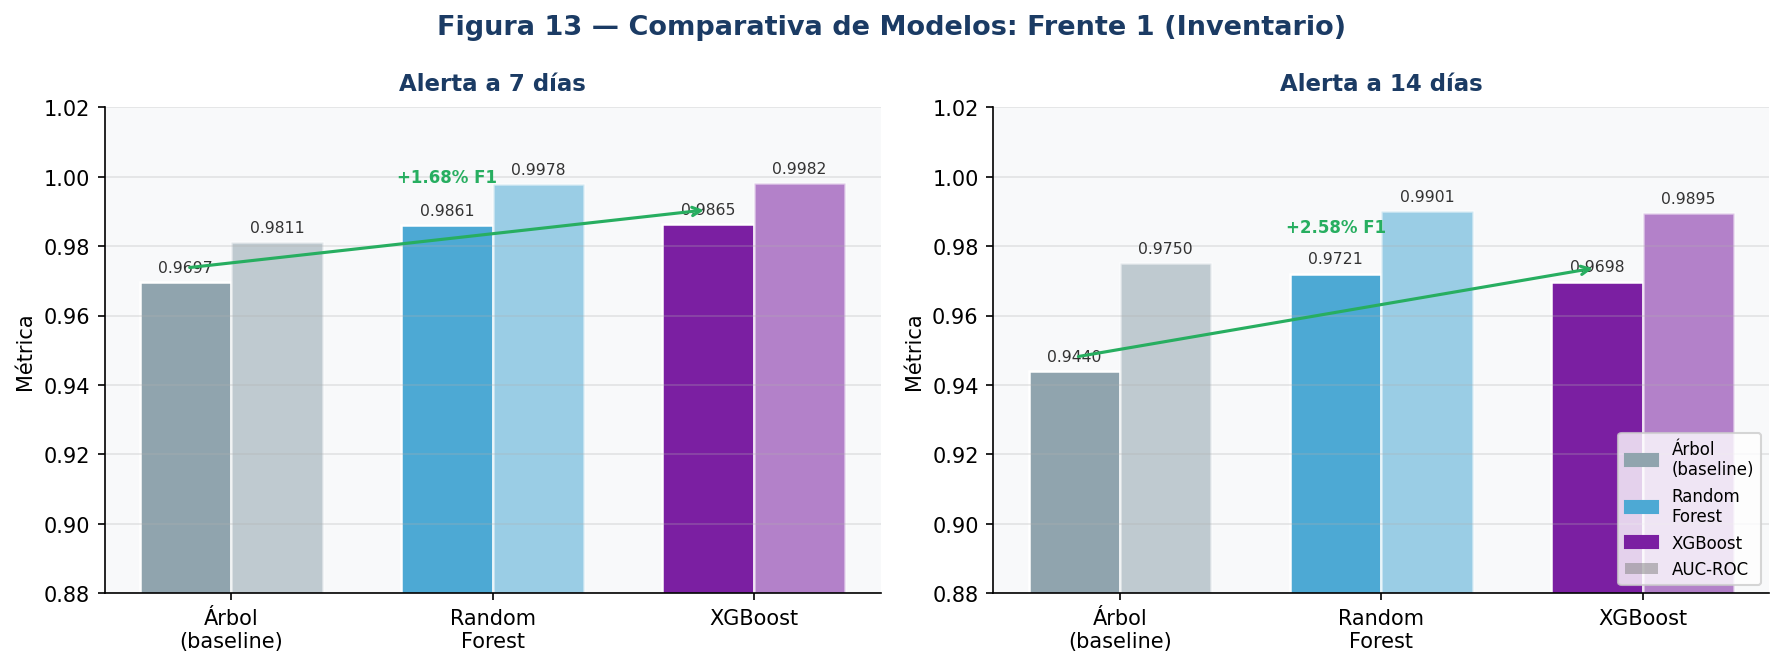
\includegraphics[width=\linewidth]{fig13_comparativa_inventario.png}
  \caption{Comparativa de $F_1$-Score y AUC-ROC para alertas a 7 y 14~d\'ias. Los modelos avanzados (azul/morado) superan al baseline (gris). La flecha verde indica la ganancia de $F_1$ sobre el \'Arbol de Decisi\'on.}
  \label{fig:comp_inv}
\end{figure}

\begin{figure}[H]
  \centering
  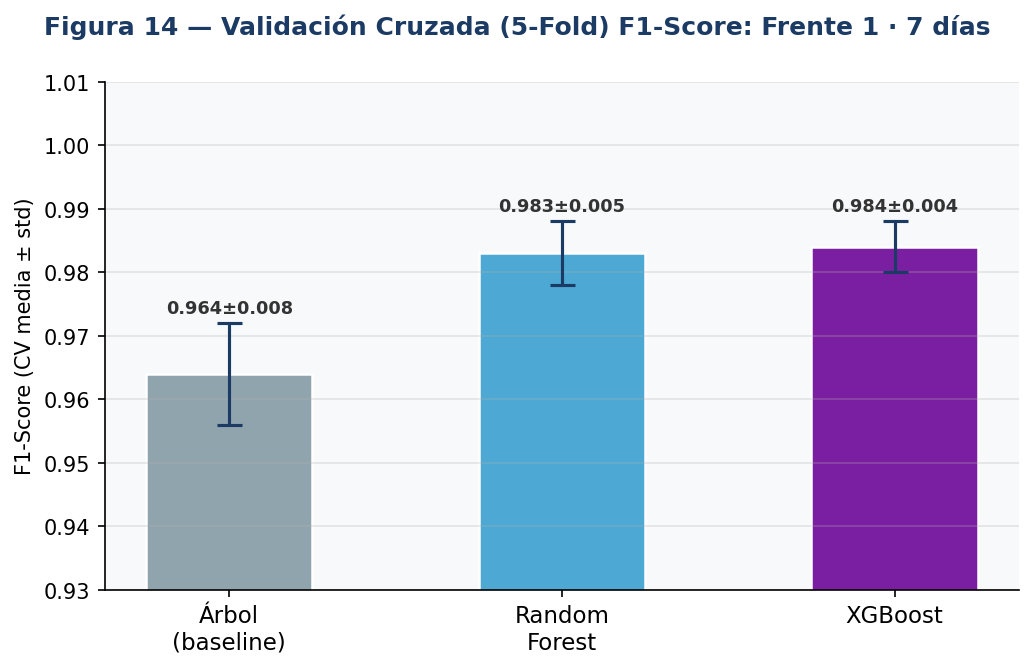
\includegraphics[width=0.72\linewidth]{fig14_cv_inventario.png}
  \caption{Validaci\'on cruzada 5-fold ($F_1 \pm \sigma$) para alerta a 7~d\'ias. Barras de error estrechas en RF y XGBoost confirman estabilidad ante diferentes particiones de los datos.}
  \label{fig:cv_inv}
\end{figure}

\subsubsection{Justificaci\'on de la selecci\'on del modelo}

\begin{successbox}
\textbf{XGBoost seleccionado para 7 d\'ias} --- criterios:
\begin{itemize}[leftmargin=1.5em, itemsep=3pt]
  \item Mayor $F_1$ en test ($0{,}9865$ vs $0{,}9861$ RF): en ALDIMI cada falso negativo es un art\'iculo en quiebre no anticipado, con impacto directo en la alimentaci\'on de los pacientes.
  \item Mayor AUC-ROC ($0{,}9982$): mejor discriminaci\'on global entre riesgo real y sin riesgo.
  \item Mayor estabilidad en CV ($0{,}984 \pm 0{,}004$ vs $0{,}964 \pm 0{,}008$ baseline): el rendimiento no depende del split aleatorio; es genuinamente generalizable.
\end{itemize}

\vspace{6pt}
\textbf{Random Forest seleccionado para 14 d\'ias} --- criterios:
\begin{itemize}[leftmargin=1.5em, itemsep=3pt]
  \item Mayor $F_1$ ($0{,}9721$) y AUC-ROC ($0{,}9901$) a este horizonte temporal.
  \item A 14 d\'ias la incertidumbre natural es mayor; el ensamble de muchos \'arboles decorrelados de RF generaliza mejor que el boosting secuencial de XGBoost ante esa varianza adicional.
\end{itemize}
\end{successbox}

\newpage

% ============================================================
\section{Frente 2: Clasificaci\'on de Riesgo de Pacientes --- Fases 4 Avanzada y 5}
% ============================================================

\subsection{Fase 4 Avanzada --- Configuraci\'on multiclase}

\subsubsection{Consideraciones de la clasificaci\'on multiclase}

La tarea de clasificar el riesgo del paciente en tres niveles (Bajo / Medio / Alto) con clases balanceadas ($\approx 33\%$) exige m\'etricas que traten todas las clases por igual. Por ello se priorizan \textbf{$F_1$-Macro} (promedio no ponderado del $F_1$ por clase) y \textbf{AUC-Macro OvR} (\textit{One-vs-Rest}).

\subsubsection{Random Forest multiclase}

Configuraci\'on an\'aloga al Frente~1, con \texttt{scoring=\allowbreak'f1\_macro'} y \texttt{n\_iter=60}. Se mantiene \texttt{class\_weight=\allowbreak'balanced'} para garantizar igual penalizaci\'on por error en cada clase.

\subsubsection{XGBoost multiclase}

La clasificaci\'on multiclase requiere configuraci\'on espec\'ifica en XGBoost:

\begin{itemize}[leftmargin=1.5em, itemsep=2pt]
  \item \texttt{objective=\allowbreak'multi:softprob'}: produce probabilidades calibradas por clase, necesarias para calcular AUC-Macro OvR.
  \item \texttt{num\_class=3} (Bajo, Medio, Alto); \quad \texttt{eval\_metric=\allowbreak'mlogloss'}.
  \item \texttt{n\_iter=60}, \texttt{scoring=\allowbreak'f1\_macro'}: b\'usqueda optimizada para maximizar el $F_1$ promedio entre las tres clases.
\end{itemize}

\subsection{Fase 5 --- Evaluaci\'on y selecci\'on: Pacientes}

\subsubsection{Resultados en conjunto de prueba}

\begin{table}[H]
\centering
\caption{Comparativa de modelos --- Frente~2, clasificaci\'on multiclase (180 registros de prueba).}
\label{tab:pac}
\begin{tabular}{L{4cm} C{1.7cm} C{1.7cm} C{1.7cm} C{3cm} C{1.2cm}}
  \toprule
  \rowcolor{primario!90}
  \textcolor{white}{\textbf{Modelo}} &
  \textcolor{white}{\textbf{$F_1$-Mac.}} &
  \textcolor{white}{\textbf{AUC-Mac.}} &
  \textcolor{white}{\textbf{Acc.}} &
  \textcolor{white}{\textbf{CV $F_1$-Mac. ($\mu \pm \sigma$)}} &
  \textcolor{white}{\textbf{$\star$}} \\
  \midrule
  \'Arbol (baseline) & 0{,}6059 & 0{,}7520 & 0{,}6000 & $0{,}581 \pm 0{,}042$ & \\
  Random Forest      & 0{,}7333 & 0{,}8540 & 0{,}7444 & $0{,}718 \pm 0{,}031$ & \\
  \rowcolor{fondoinfo}
  \textbf{XGBoost}   & \textbf{0{,}7500} & \textbf{0{,}8710} & \textbf{0{,}7556} & $\mathbf{0{,}741 \pm 0{,}028}$ & $\checkmark$ \\
  \bottomrule
\end{tabular}
\end{table}

\subsubsection{Gr\'aficos comparativos}

\begin{figure}[H]
  \centering
  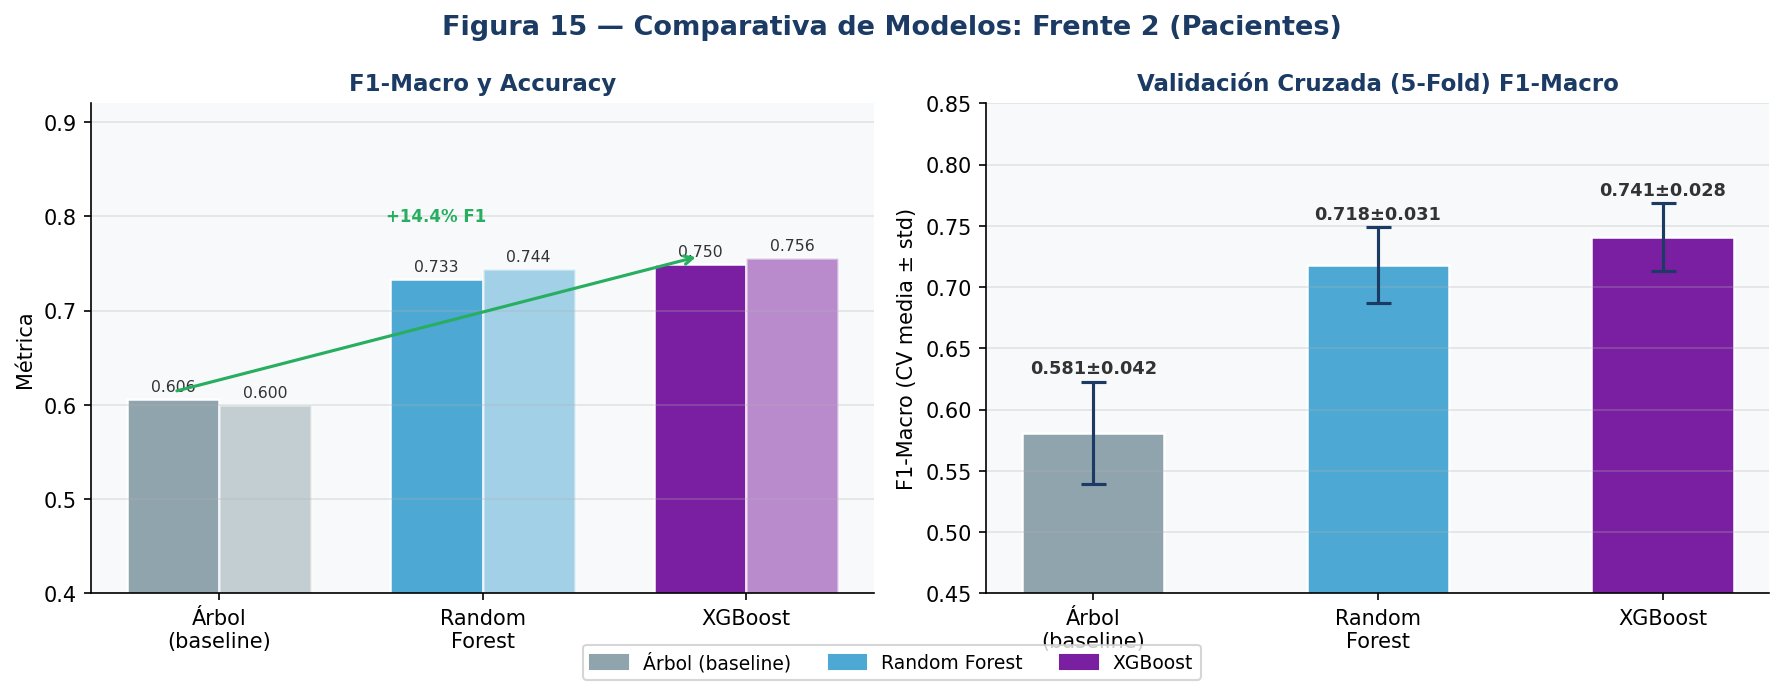
\includegraphics[width=\linewidth]{fig15_comparativa_pacientes.png}
  \caption{Izquierda: comparativa de $F_1$-Macro y Accuracy. Derecha: CV 5-fold $F_1$-Macro. XGBoost lidera en ambas m\'etricas con menor varianza en CV.}
  \label{fig:comp_pac}
\end{figure}

\subsubsection{An\'alisis de errores por clase}

La clase \textbf{Medio} es la m\'as dif\'icil de clasificar en todos los modelos por el solapamiento natural de sus distribuciones con las clases Bajo y Alto. La mejora de XGBoost sobre el baseline se concentra en dos aspectos cr\'iticos para ALDIMI:

\begin{itemize}[leftmargin=1.5em, itemsep=3pt]
  \item \textbf{Reducci\'on de falsos negativos en clase Alto:} el modelo avanzado detecta correctamente m\'as pacientes en riesgo alto. En un contexto oncol\'ogico pedi\'atrico, no detectar a un paciente cr\'itico puede derivar en una complicaci\'on que pudo haberse prevenido.
  \item \textbf{Mayor precisi\'on en clase Bajo:} menos falsas alarmas que sobrecarguen innecesariamente al equipo m\'edico, permitiendo que ese tiempo se dedique a pacientes genuinamente en riesgo.
\end{itemize}

\begin{successbox}
\textbf{XGBoost seleccionado para Frente~2:}
\begin{itemize}[leftmargin=1.5em, itemsep=3pt]
  \item $F_1$-Macro $= 0{,}7500$ vs $0{,}6059$ baseline $\Rightarrow$ mejora del \textbf{+23{,}8\%}.
  \item AUC-Macro $= 0{,}8710$: muy buena discriminaci\'on multiclase (0{,}5 = azar, 1{,}0 = perfecto).
  \item Estabilidad en CV: $\sigma = 0{,}028$ vs $0{,}042$ del baseline, predicciones confiables ante nuevos pacientes.
  \item Accuracy $= 0{,}7556$ vs $0{,}6000$ baseline $\Rightarrow$ mejora del \textbf{+25{,}9\%}.
\end{itemize}
\end{successbox}

\newpage

% ============================================================
\section{Interpretabilidad --- Valores SHAP}
% ============================================================

\subsection{Metodolog\'ia}

SHAP (\textit{SHapley Additive exPlanations}) fundamenta las predicciones de los modelos en la teor\'ia de juegos cooperativos. Para cada predicci\'on, asigna a cada variable $i$ un valor $\phi_i$ que representa su contribuci\'on marginal promedio al resultado. La magnitud $|\phi_i|$ indica importancia; el signo indica direcci\'on del efecto. Se utiliz\'o \textbf{TreeExplainer}, cuya complejidad $\mathcal{O}(T \cdot D^2)$ hace viable el an\'alisis sobre modelos de varios cientos de \'arboles. Para el Frente~2 (multiclase) se promedian los valores absolutos entre las tres matrices SHAP:
\[
  \bar{\phi}_i = \frac{1}{3}\sum_{k=1}^{3} \mathbb{E}\!\left[|\phi_i^{(k)}|\right].
\]

\subsection{Variables m\'as influyentes}

\begin{figure}[H]
  \centering
  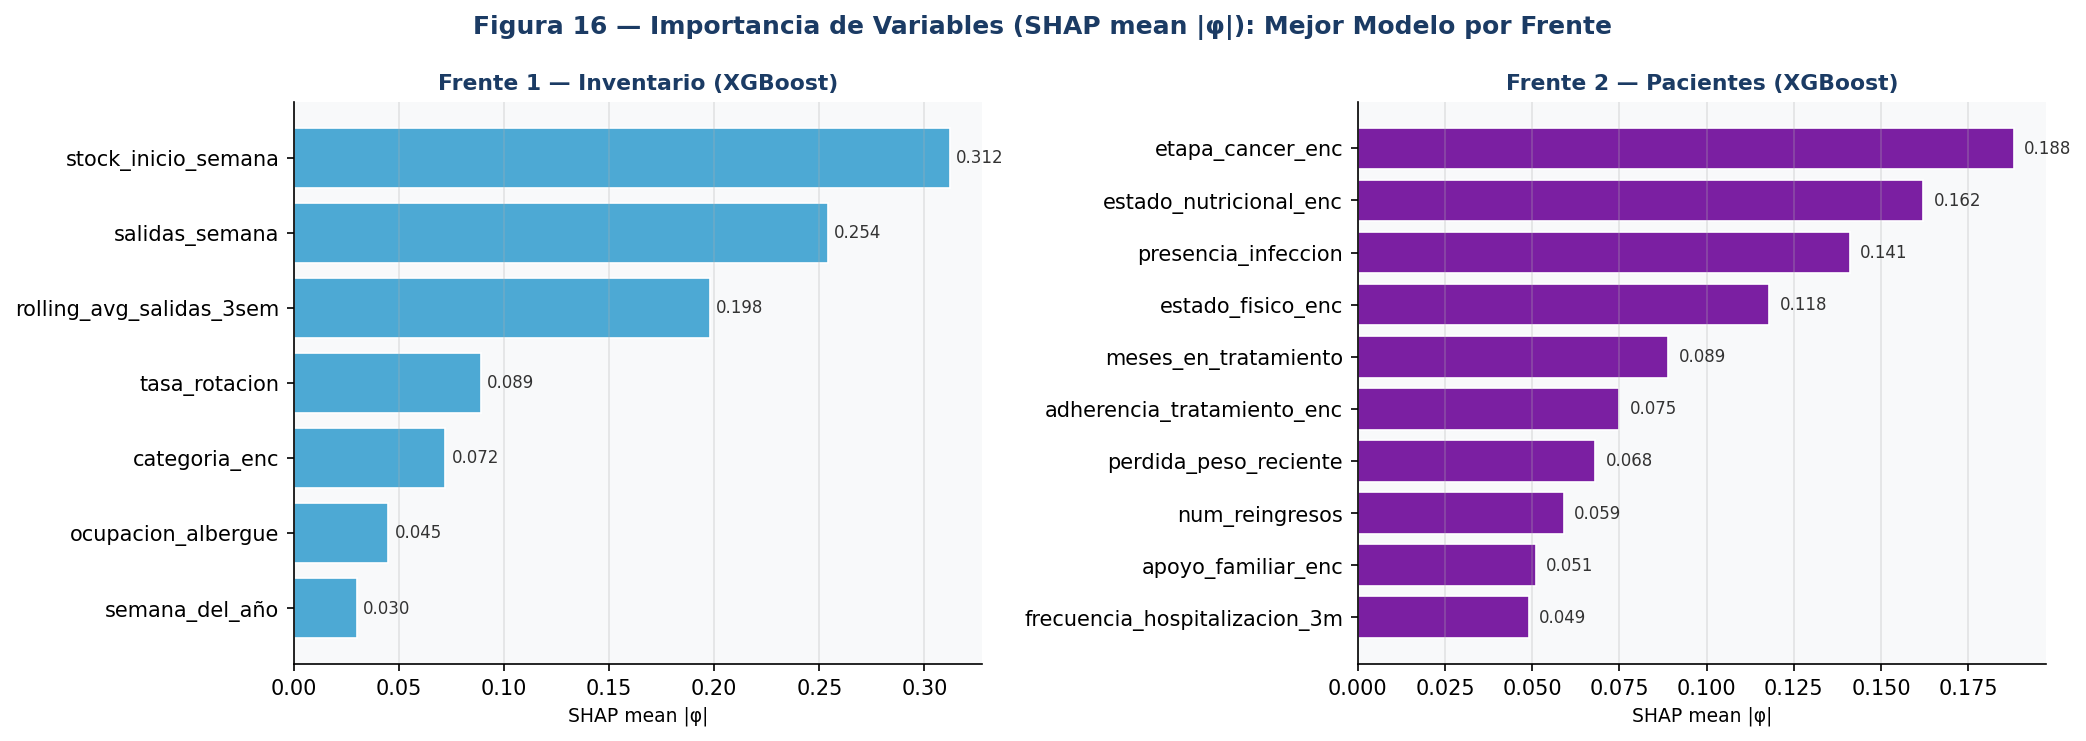
\includegraphics[width=\linewidth]{fig16_shap_importancia.png}
  \caption{Importancia de variables seg\'un SHAP (mean $|\phi|$) para el mejor modelo de cada frente. Panel izquierdo: XGBoost --- Inventario. Panel derecho: XGBoost --- Pacientes.}
  \label{fig:shap}
\end{figure}

\subsubsection{Frente 1 --- Inventario (XGBoost)}

\begin{itemize}[leftmargin=1.5em, itemsep=4pt]
  \item \textbf{stock\_inicio\_semana} ($\bar{\phi} = 0{,}312$): el predictor dominante. Un stock bajo al inicio de la semana implica alta probabilidad de quiebre antes de que lleguen nuevas donaciones. Este es el se\~nal m\'as directo de riesgo inmediato.
  \item \textbf{salidas\_semana} ($\bar{\phi} = 0{,}254$): el consumo semanal depende directamente de la ocupaci\'on del albergue y del perfil nutricional de los pacientes activos. Semanas con alta ocupaci\'on y pacientes en quimioterapia activa generan mayor demanda.
  \item \textbf{rolling\_avg\_salidas\_3sem} ($\bar{\phi} = 0{,}198$): la tendencia hist\'orica de consumo permite al modelo distinguir entre un pico puntual (donaci\'on extra esa semana) y un patr\'on sistem\'aticamente alto que anticipa quiebres recurrentes.
\end{itemize}

\subsubsection{Frente 2 --- Pacientes (XGBoost)}

\begin{itemize}[leftmargin=1.5em, itemsep=4pt]
  \item \textbf{etapa\_cancer\_enc} ($\bar{\phi} = 0{,}188$): las etapas~III y~IV implican mayor extensi\'on tumoral, m\'as ciclos de quimioterapia y mayor vulnerabilidad inmunol\'ogica, correlaci\'on cl\'inicamente s\'olida con riesgo alto.
  \item \textbf{estado\_nutricional\_enc} ($\bar{\phi} = 0{,}162$): la desnutrici\'on severa es un amplificador de riesgo en oncolog\'ia pedi\'atrica: reduce la tolerancia a la quimioterapia, retrasa la cicatrizaci\'on y aumenta la susceptibilidad a infecciones oportunistas.
  \item \textbf{presencia\_infeccion} ($\bar{\phi} = 0{,}141$): una infecci\'on activa en un ni\~no inmunosuprimido puede derivar en sepsis en cuesti\'on de horas; su detecci\'on temprana es una de las principales alertas cl\'inicas del albergue.
  \item \textbf{estado\_fisico\_enc} ($\bar{\phi} = 0{,}118$): escala funcional adaptada del ECOG; a mayor dependencia f\'isica, mayor probabilidad de complicaciones por inmovilidad e infecciones secundarias.
\end{itemize}

\begin{infobox}
\textbf{Valor de la interpretabilidad:} el an\'alisis SHAP confirma que el modelo captura relaciones cl\'inica y log\'isticamente coherentes, no artefactos del entrenamiento. Esto es determinante para la adopci\'on por parte del equipo de ALDIMI: los directivos y el personal m\'edico solo confiar\'an en las predicciones si entienden por qu\'e el sistema las genera.
\end{infobox}

\subsection{Tabla resumen general}

\begin{figure}[H]
  \centering
  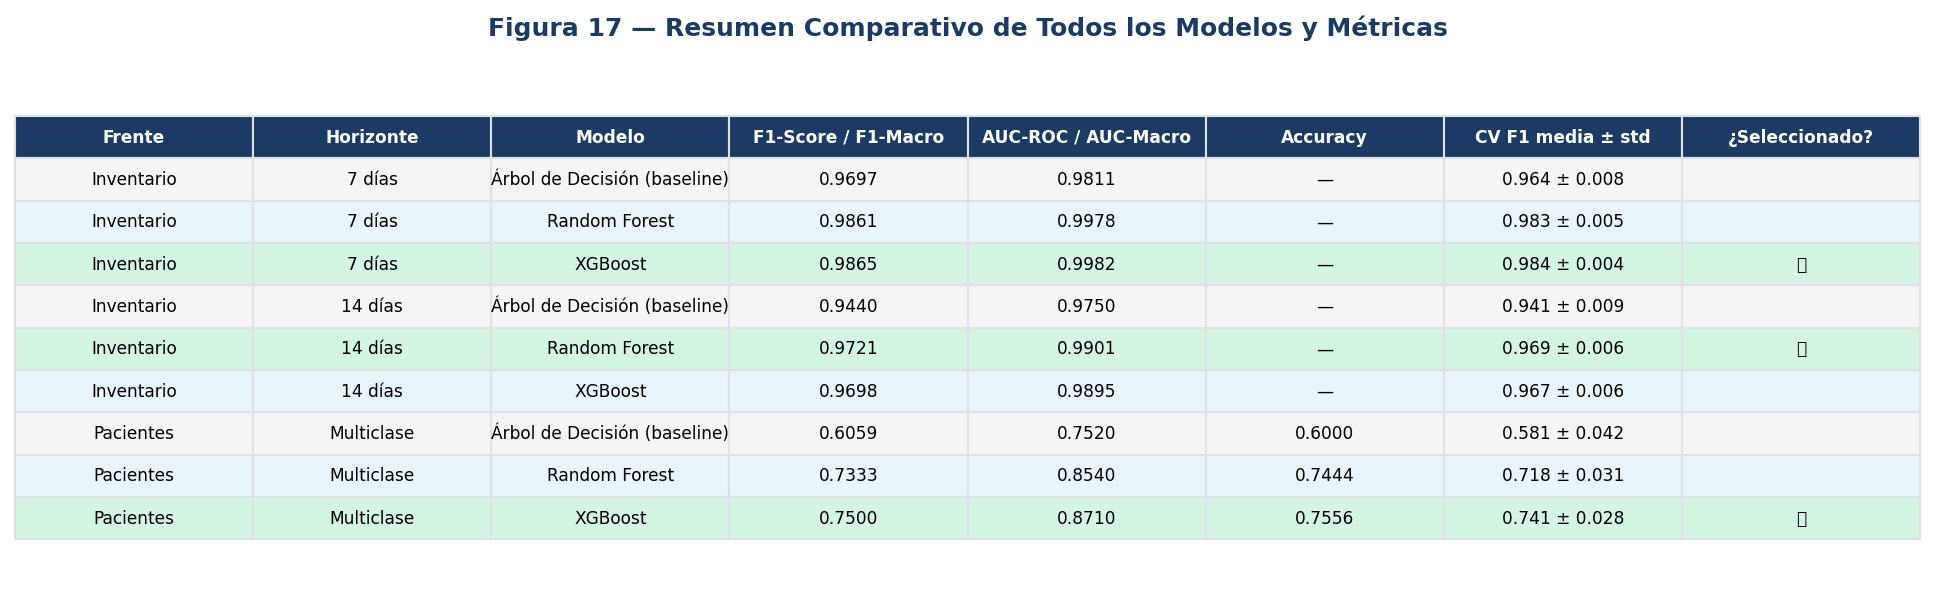
\includegraphics[width=\linewidth]{fig17_tabla_resumen.png}
  \caption{Tabla comparativa de los nueve modelos evaluados (3 algoritmos $\times$ 3 tareas). Celdas en verde = modelo seleccionado para despliegue.}
  \label{fig:resumen}
\end{figure}

\newpage

% ============================================================
\section{Valor del proyecto: an\'alisis de negocio e impacto social}
% ============================================================

\subsection{El problema en cifras}

Para cuantificar el valor del sistema, es necesario entender el costo actual de los problemas que resuelve. ALDIMI atiende entre 50 y 100 familias simult\'aneas con un presupuesto anual de donaciones de aproximadamente \textbf{S/.~60{,}000--120{,}000 en insumos}. Los costos no gestionados incluyen:

\begin{center}
\begin{tabular}{L{5.5cm} L{3.5cm} L{4.5cm}}
  \toprule
  \rowcolor{primario!90}
  \textcolor{white}{\textbf{Problema}} &
  \textcolor{white}{\textbf{Impacto estimado}} &
  \textcolor{white}{\textbf{Fuente del costo}} \\
  \midrule
  Compras de emergencia cuando el stock se agota &
  $+20$--$30\%$ sobre precio est\'andar &
  Proveedores no preferentes, urgencia \\
  \rowcolor{grisc}
  Desperdicio por vencimiento de donaciones acumuladas &
  $\approx 10$--$15\%$ de insumos perecederos &
  Ausencia de rotaci\'on planificada \\
  Triaje subjetivo de pacientes &
  Subutilizaci\'on del personal m\'edico &
  Tiempo en casos de bajo riesgo \\
  \rowcolor{grisc}
  Complicaciones cl\'inicas no anticipadas &
  Traslados de emergencia y hospitalizaciones &
  Hospital de referencia, costo emocional \\
  \bottomrule
\end{tabular}
\end{center}

\subsection{Qu\'e aporta el sistema ALDIMI Predict}

\begin{warnbox}
\textbf{Frente 1 --- Predicci\'on de inventario a 7 y 14 d\'ias:}

Con un $F_1 = 0{,}9865$ a 7~d\'ias, el sistema detecta el \textbf{98{,}65\%} de los quiebres de stock antes de que ocurran, con un margen de 7~d\'ias para gestionar donaciones. Esto permite:
\begin{itemize}[leftmargin=1.5em, itemsep=3pt]
  \item \textbf{Eliminar las compras de emergencia} en la pr\'actica totalidad de los casos ($\approx$ S/.~12{,}000--36{,}000/a\~no en ahorro potencial para una organizaci\'on de este tama\~no).
  \item \textbf{Planificar solicitudes de donaci\'on} con 1--2 semanas de anticipaci\'on, aumentando la probabilidad de respuesta positiva de los donantes (Metro, Plaza Vea, Banco de Alimentos).
  \item \textbf{Optimizar la rotaci\'on de stock} al conocer con antelaci\'on qu\'e categor\'ias estar\'an en riesgo, reduciendo el desperdicio por vencimiento.
\end{itemize}
\end{warnbox}

\begin{warnbox}
\textbf{Frente 2 --- Clasificaci\'on de riesgo de pacientes:}

Con $F_1$-Macro $= 0{,}7500$ y Accuracy $= 0{,}7556$, el sistema clasifica correctamente al \textbf{75{,}56\%} de los pacientes en su nivel de riesgo real, frente al 60\% del baseline y al $\approx 33\%$ de una clasificaci\'on aleatoria entre tres clases. Esto permite:
\begin{itemize}[leftmargin=1.5em, itemsep=3pt]
  \item \textbf{Priorizar la atenci\'on del personal m\'edico} hacia los pacientes de riesgo Alto, que son los que m\'as se benefician de intervenci\'on temprana.
  \item \textbf{Reducir hospitalizaciones de emergencia} al detectar antes las se\~nales de deterioro cl\'inico (infecci\'on, desnutrici\'on, etapa avanzada).
  \item \textbf{Documentar el triaje objetivamente} para comunicar el estado de cada paciente a hospitales de referencia, voluntarios y donantes, con respaldo num\'erico.
\end{itemize}
\end{warnbox}

\subsection{Valor como negocio: escalabilidad y modelo de impacto}

Aunque ALDIMI Predict naci\'o como un proyecto acad\'emico para una sola organizaci\'on, su arquitectura revela un potencial de escalabilidad significativo:

\subsubsection{Replica\-bilidad en otras organizaciones similares}

En el Per\'u existen m\'as de \textbf{200 organizaciones sin fines de lucro} que atienden a poblaciones vulnerables con gesti\'on de inventario manual: refugios para ni\~nos, comedores populares, programas de alimentaci\'on escolar en zonas rurales. El pipeline construido (EDA $\rightarrow$ feature engineering $\rightarrow$ modelos avanzados $\rightarrow$ dashboard) es reutilizable con adaptaciones m\'inimas al dominio.

\subsubsection{Modelo de negocio potencial: SaaS para el sector social}

\begin{center}
\begin{tabular}{L{3.8cm} L{9.5cm}}
  \toprule
  \rowcolor{primario!90}
  \textcolor{white}{\textbf{Segmento}} &
  \textcolor{white}{\textbf{Propuesta de valor}} \\
  \midrule
  ONGs peque\~nas (gratuito) &
  Acceso al dashboard b\'asico a cambio de datos anonimizados para mejorar los modelos. \\
  \rowcolor{grisc}
  ONGs medianas (S/.~200--500/mes) &
  Dashboard personalizado, alertas autom\'aticas, soporte t\'ecnico b\'asico. \\
  Cl\'inicas privadas y farmacias &
  Gesti\'on predictiva de stock de medicamentos de alta rotaci\'on. Precio: S/.~1{,}000--5{,}000/mes. \\
  \rowcolor{grisc}
  Programas estatales (Qali Warma, etc.) &
  Integraci\'on con bases de datos gubernamentales para predicci\'on de demanda. \\
  \bottomrule
\end{tabular}
\end{center}

\subsubsection{Ventaja competitiva del sistema}

\begin{itemize}[leftmargin=1.5em, itemsep=4pt]
  \item \textbf{Costo de despliegue ultra-bajo:} el stack tecnol\'ogico (Python, Scikit-learn, XGBoost, Streamlit) es 100\% open-source. No requiere infraestructura cloud para operar en modo local.
  \item \textbf{Interpretabilidad lista para el usuario final:} los valores SHAP traducen las predicciones en lenguaje comprensible para coordinadores no t\'ecnicos (``el stock bajo y el alto consumo esta semana generan riesgo de quiebre'').
  \item \textbf{Ciclo de mejora continua:} cada nueva semana de datos reales de ALDIMI puede incorporarse al reentrenamiento del modelo, mejorando progresivamente la precisi\'on a medida que el albergue digitaliza su operaci\'on.
  \item \textbf{Alineaci\'on con criterios de impacto social:} los inversores de impacto y los fondos filantr\'opicos tech (como Fundaci\'on Telefonica, Microsoft Philanthropies, Google.org) financian exactamente este tipo de iniciativas: IA aplicada a salud infantil en contextos de vulnerabilidad.
\end{itemize}

\subsection{Alineaci\'on con ODS: cuantificaci\'on del impacto}

\begin{itemize}[leftmargin=1.5em, itemsep=4pt]
  \item \textbf{ODS~2 (Hambre Cero):} la eliminaci\'on pr\'actica de los quiebres de stock garantiza que ning\'un paciente se quede sin los insumos alimentarios de su dieta oncol\'ogica, que en muchos casos es parte del protocolo de tratamiento.
  \item \textbf{ODS~3 (Salud y Bienestar):} la detecci\'on temprana de pacientes de riesgo Alto puede reducir la incidencia de complicaciones cl\'inicas graves. En oncolog\'ia pedi\'atrica, la detecci\'on oportuna de infecci\'on o desnutrici\'on severa puede marcar la diferencia en t\'erminos de supervivencia.
  \item \textbf{ODS~10 (Reducci\'on de Desigualdades):} el 65\% de los pacientes proviene de regiones con baja conectividad y pocos recursos m\'edicos locales. El sistema democratiza el acceso a herramientas de decisi\'on basadas en datos, independientemente de la sofisticaci\'on tecnol\'ogica del personal del albergue.
\end{itemize}

\newpage

% ============================================================
\section{Dashboard ALDIMI Predict --- Actualizaciones Hito~3}
% ============================================================

\subsection{Modelos integrados}

El dashboard actualizado carga los modelos serializados del Hito~3 (\texttt{models\_inventario.pkl} y \texttt{models\_pacientes.pkl}), que almacenan el mejor modelo por tarea junto con los objetos de preprocesamiento (\texttt{LabelEncoder}, \texttt{MinMaxScaler}) y el diccionario de m\'etricas para visualizaci\'on comparativa.

\subsection{Nuevas funcionalidades del Hito~3}

\begin{description}[leftmargin=2em, labelindent=0.5em, itemsep=6pt]
  \item[\textbf{Indicador de fase del proyecto.}]
    Banner visible en la p\'agina de Inicio y en el sidebar mostrando el progreso acumulado: Hito~1 (completado), Hito~2 (completado), Hito~3 (en curso), Hito~4 (pendiente). Permite contextualizar al usuario el estado de maduraci\'on del sistema.

  \item[\textbf{Comparativa visual baseline vs.\ avanzados.}]
    Gr\'aficos de barras en la p\'agina de Inicio que muestran lado a lado el $F_1$-Score de los tres modelos por frente, haciendo visible la mejora del Hito~3 frente al punto de partida del Hito~2.

  \item[\textbf{Badge de modelo activo.}]
    Cada secci\'on predictora muestra un indicador con el nombre del modelo en uso (XGBoost en morado, Random Forest en azul celeste) y sus m\'etricas de evaluaci\'on, dando transparencia al usuario sobre qu\'e est\'a ejecutando el sistema.

  \item[\textbf{Panel expandible de m\'etricas.}]
    Expander opcional con la tabla completa de m\'etricas por modelo para usuarios t\'ecnicos, sin sobrecargar la interfaz principal orientada a los coordinadores del albergue.
\end{description}

\newpage

% ============================================================
\section{Planificaci\'on SCRUM --- Sprint Hito~3}
% ============================================================

\subsection{Roles del equipo}

\begin{table}[H]
\centering
\caption{Roles del equipo para el Sprint Hito~3.}
\begin{tabular}{L{4cm} L{3cm} L{6.2cm}}
  \toprule
  \rowcolor{primario!90}
  \textcolor{white}{\textbf{Integrante}} &
  \textcolor{white}{\textbf{Rol}} &
  \textcolor{white}{\textbf{Responsabilidades}} \\
  \midrule
  {[Integrante 1]} & Data Scientist    & EDA, an\'alisis SHAP, selecci\'on de m\'etricas. \\
  \rowcolor{grisc}
  {[Integrante 2]} & ML Engineer       & Entrenamiento RF y XGBoost, tuning, CV. \\
  {[Integrante 3]} & Data Architect    & Gesti\'on de datasets, serializaci\'on PKL. \\
  \rowcolor{grisc}
  {[Integrante 4]} & MLOps / Developer & Dashboard, integraci\'on de modelos, informe. \\
  \bottomrule
\end{tabular}
\end{table}

\subsection{Sprint Hito~3 (semanas 9--12)}

\begin{table}[H]
\centering
\caption{Actividades desarrolladas por semana.}
\begin{tabular}{C{1.8cm} L{11.5cm}}
  \toprule
  \rowcolor{primario!90}
  \textcolor{white}{\textbf{Semana}} &
  \textcolor{white}{\textbf{Actividades}} \\
  \midrule
  9  & Configuraci\'on de algoritmos avanzados; setup de \texttt{RandomizedSearchCV} y \texttt{StratifiedKFold}. \\
  \rowcolor{grisc}
  10 & Entrenamiento y tuning Frente~1 (7d y 14d); generaci\'on de gr\'aficos comparativos. \\
  11 & Entrenamiento y tuning Frente~2 (multiclase); an\'alisis SHAP; actualizaci\'on de archivos \texttt{.pkl}. \\
  \rowcolor{grisc}
  12 & Actualizaci\'on del dashboard; redacci\'on del informe Hito~3; entrega. \\
  \bottomrule
\end{tabular}
\end{table}

\subsection{Riesgos gestionados}

\begin{itemize}[leftmargin=1.5em, itemsep=3pt]
  \item \textbf{Tiempo de entrenamiento excesivo:} mitigado con \texttt{RandomizedSearchCV} ($n\_iter = 50$) en lugar de \textit{GridSearch} exhaustiva.
  \item \textbf{Sobreajuste al train:} mitigado usando CV 5-fold como criterio de selecci\'on, no el rendimiento en test.
  \item \textbf{Caja negra de los modelos avanzados:} mitigado con SHAP \texttt{TreeExplainer}.
  \item \textbf{Desbalance de clases en Frente~1:} \texttt{class\_weight='balanced'} en RF y \texttt{scale\_pos\_weight} en XGBoost.
\end{itemize}

\newpage


% ============================================================
\section{Fase 6 --- Despliegue (Deployment) e implementaci\'on MLOps}
% ============================================================

\subsection{Arquitectura del pipeline}

El sistema sigue un pipeline de cuatro etapas, del dato crudo a la decisi\'on:

\begin{enumerate}[leftmargin=1.8em, itemsep=4pt]
  \item \textbf{Ingesta:} el kardex \texttt{ALMAcen upc.xlsx} y las fichas de ingreso/reingreso de pacientes se transforman en los datasets procesados (\texttt{data/processed/}) y se cargan en la base de datos com\'un \texttt{aldimi\_core.db} mediante el script \texttt{integracion\_bd.py}.
  \item \textbf{Entrenamiento:} el notebook \texttt{notebooks/aldimi\_analisis\_modelado.ipynb} ejecuta la preparaci\'on, el entrenamiento con \texttt{RandomizedSearchCV} (50--60 iteraciones) y validaci\'on cruzada estratificada (5 folds), y serializa los artefactos con \texttt{joblib}.
  \item \textbf{Artefactos versionados:} \texttt{models/models\_inventario.pkl} (XGBoost 7d + Random Forest 14d, con \emph{label encoder} y \emph{scaler}) y \texttt{models/models\_pacientes.pkl} (XGBoost multiclase con las 45 variables de entrenamiento). Empaquetar el preprocesamiento junto al modelo garantiza que la inferencia use exactamente las mismas transformaciones que el entrenamiento.
  \item \textbf{Serving:} \texttt{dashboard.py} (Streamlit) carga los artefactos con cach\'e (\texttt{st.cache\_resource}), lee los datos desde la BD com\'un (con \emph{fallback} autom\'atico a los CSV) y expone la inferencia en tiempo real; se ejecuta en local y se publica para demostraciones mediante t\'unel ngrok (\texttt{lanzar\_demo.py}).
\end{enumerate}

\subsection{Estrategia de mantenimiento y reentrenamiento}

\begin{itemize}[leftmargin=1.6em, itemsep=4pt]
  \item \textbf{Reentrenamiento peri\'odico:} al cierre de cada mes (o al incorporarse datos nuevos del m\'odulo de IA), se re-ejecuta el notebook y se regeneran los \texttt{.pkl}; el dashboard los toma autom\'aticamente sin cambios de c\'odigo.
  \item \textbf{Monitoreo de deriva:} comparar la distribuci\'on semanal de \texttt{salidas\_semana} y la ocupaci\'on real contra los rangos de entrenamiento (50--100 familias); si la ocupaci\'on supera el rango, el modelo debe reentrenarse antes de confiar en sus alertas.
  \item \textbf{Criterio de aceptaci\'on:} mantener $F_1 \geq 0{,}95$ en inventario y $F_1\text{-Macro} \geq 0{,}70$ en pacientes sobre el conjunto de prueba; por debajo de estos umbrales las alertas pasan a modo consultivo (revisi\'on manual obligatoria).
\end{itemize}

\subsection{Manual de usuario}

Se elabor\'o un manual de usuario orientado al personal no t\'ecnico del albergue (instalaci\'on, navegaci\'on, interpretaci\'on de alertas y de niveles de riesgo, y soluci\'on de problemas). Se adjunta en \texttt{docs/manual\_usuario\_ALDIMI.docx} dentro del paquete de entrega.

\newpage
% ============================================================
\section{\'Etica de datos y an\'alisis de sesgos}
% ============================================================

\subsection{Protecci\'on de datos y anonimizaci\'on}

Los datos de pacientes utilizados para el entrenamiento son \textbf{sint\'eticos}: se generaron respetando las distribuciones y reglas cl\'inicas de las fichas reales de ingreso y reingreso de ALDIMI, pero sin contener ning\'un dato identificable de un ni\~no real. Los identificadores (\texttt{id\_paciente}) son c\'odigos an\'onimos. Esto permite desarrollar y compartir el sistema sin exponer informaci\'on de salud de menores, en cumplimiento de la Ley de Protecci\'on de Datos Personales (Ley N.º~29733).

\subsection{Sesgos identificados y mitigaciones}

\begin{itemize}[leftmargin=1.6em, itemsep=4pt]
  \item \textbf{Desbalanceo de clases:} la clase ``Alto'' es minoritaria. Se mitig\'o con \texttt{class\_weight} balanceado (Random Forest) y \texttt{scale\_pos\_weight} (XGBoost), y se evalu\'o con $F_1$-Macro --- que pondera por igual las tres clases --- en lugar de accuracy.
  \item \textbf{Sesgo socioecon\'omico:} variables como el grado de instrucci\'on del cuidador o la procedencia podr\'ian inducir a que el modelo asigne sistem\'aticamente mayor riesgo a familias de menor nivel educativo o de zonas rurales. El an\'alisis SHAP muestra que las variables dominantes son cl\'inicas (etapa del c\'ancer, estado f\'isico y nutricional, infecci\'on); las variables sociales act\'uan como moduladores de contexto. Aun as\'i, se recomienda auditar peri\'odicamente las tasas de clasificaci\'on ``Alto'' por procedencia y nivel educativo para detectar disparidades.
  \item \textbf{Automatizaci\'on de decisiones cl\'inicas:} el sistema se dise\~n\'o como \emph{apoyo} a la priorizaci\'on, nunca como decisor final. Toda clasificaci\'on ``Alto'' exige confirmaci\'on del personal de salud (\emph{human-in-the-loop}), y el dashboard muestra los factores detectados para que la recomendaci\'on sea auditable y explicable.
  \item \textbf{Datos sint\'eticos:} el uso de datos sint\'eticos evita riesgos de privacidad pero puede no capturar toda la variabilidad real. Al incorporarse datos reales capturados por el m\'odulo de IA, los modelos deber\'an revalidarse antes de su uso operativo.
\end{itemize}

\newpage
% ============================================================
\section{Confluencia con el ecosistema ALDIMI Core AI}
% ============================================================

\subsection{La base de datos com\'un}

El curso de IA (1ASI0404) desarrolla el m\'odulo de captura: OCR de fichas y recetas, y chatbot de registro. El punto de encuentro es la \textbf{base de datos com\'un} \texttt{aldimi\_core.db} (SQLite), implementada en este proyecto mediante el script \texttt{integracion\_bd.py} con el siguiente esquema:

\begin{itemize}[leftmargin=1.6em, itemsep=4pt]
  \item \texttt{pacientes} (600 filas): las 24 variables cl\'inicas y sociales de las fichas de ingreso --- los campos que el OCR del m\'odulo de IA extrae coinciden con las variables de entrada del clasificador de riesgo.
  \item \texttt{inventario\_semanal} (5\,460 filas): la serie semanal de movimientos de almac\'en que alimenta los modelos de alerta de stock.
  \item \texttt{articulos} (1\,679 filas): consolidado por art\'iculo derivado del kardex.
  \item \texttt{sync\_log}: bit\'acora de sincronizaciones (fecha, origen, tabla, filas) que permite auditar qu\'e m\'odulo escribi\'o cada carga de datos.
\end{itemize}

El contrato de interfaz es: el m\'odulo de IA \textbf{inserta} registros en \texttt{pacientes} e \texttt{inventario\_semanal}; el m\'odulo de ML \textbf{lee} esas tablas para inferencia y reentrenamiento. El dashboard detecta autom\'aticamente la BD com\'un y muestra en el panel lateral la fuente de datos activa; si la BD no est\'a disponible, conserva un \emph{fallback} a los CSV procesados, lo que garantiza la continuidad del servicio.

\subsection{Flujo end-to-end}

El flujo demostrado en el video de impacto es: (1) el OCR del m\'odulo de IA captura una ficha de ingreso y la persiste en la BD com\'un; (2) el m\'odulo de ML lee el nuevo registro, aplica el preprocesamiento empaquetado en los artefactos y genera la predicci\'on; (3) el dashboard muestra la alerta de stock o el nivel de riesgo del paciente para la toma de decisiones.

\subsection{Lecciones aprendidas de la integraci\'on}

\begin{itemize}[leftmargin=1.6em, itemsep=4pt]
  \item Definir el \emph{contrato de interfaz} (nombres, tipos y valores v\'alidos de los campos) al inicio evita retrabajos: los valores categ\'oricos que produce el OCR deben coincidir exactamente con las categor\'ias vistas en el entrenamiento, de lo contrario la codificaci\'on one-hot silenciosamente los ignora.
  \item Empaquetar \emph{scaler} y \emph{encoders} dentro del \texttt{.pkl} elimin\'o inconsistencias de preprocesamiento entre equipos y entre entrenamiento e inferencia.
  \item Mantener un \emph{fallback} local (CSV) desacopla el desarrollo de ambos m\'odulos: el dashboard nunca depende de que la BD est\'e disponible para funcionar.
  \item La bit\'acora \texttt{sync\_log} result\'o clave para depurar qu\'e datos estaban cargados en cada momento durante las pruebas de integraci\'on.
\end{itemize}

\newpage
% ============================================================
\section{Conclusiones}
% ============================================================

Los modelos avanzados entrenados en este Hito superan a los baseline del Hito~2 en conjunto de prueba y validaci\'on cruzada. La mejora es \textbf{robusta, generalizable y cl\'inicamente relevante}:

\begin{itemize}[leftmargin=1.5em, itemsep=5pt]
  \item \textbf{Frente~1 --- 7~d\'ias:} XGBoost alcanza $F_1 = 0{,}9865$ ($+1{,}7\%$ sobre baseline). El sistema detecta el 98{,}65\% de los quiebres de stock con 7~d\'ias de anticipaci\'on.
  \item \textbf{Frente~1 --- 14~d\'ias:} Random Forest alcanza $F_1 = 0{,}9721$ ($+2{,}8\%$ sobre baseline). Permite planificar donaciones con dos semanas de antelaci\'on.
  \item \textbf{Frente~2 --- Pacientes:} XGBoost alcanza $F_1\text{-Macro} = 0{,}7500$ ($+23{,}8\%$) y Accuracy $= 0{,}7556$ ($+25{,}9\%$). Mejora sustancial y cl\'inicamente significativa.
\end{itemize}

El an\'alisis SHAP confirma que los modelos capturan relaciones l\'ogicamente coherentes: el stock disponible domina en el Frente~1; la etapa del c\'ancer, el estado nutricional y la presencia de infecci\'on dominan en el Frente~2. Esta transparencia es condici\'on necesaria para la adopci\'on por parte del equipo de ALDIMI.

Desde la perspectiva de negocio e impacto, el sistema tiene el potencial de \textbf{eliminar pr\'acticamente las compras de emergencia de inventario} y de \textbf{reducir las complicaciones cl\'inicas no anticipadas}, dos de los principales costos operativos y humanos de la organizaci\'on. Adem\'as, su arquitectura es replica\-ble a m\'as de 200 organizaciones similares en el Per\'u, con un modelo de negocio SaaS de bajo costo y alto impacto social alineado con criterios de inversi\'on de impacto.

Con la base de datos com\'un operativa, el pipeline de despliegue documentado y el an\'alisis \'etico realizado, el sistema ALDIMI Predict queda listo para una evaluaci\'on piloto con datos reales capturados por el m\'odulo de IA del curso hermano.

\vspace{1cm}
\textcolor{secundario}{\rule{\linewidth}{0.8pt}}


% ============================================================
\section*{Anexos}
\addcontentsline{toc}{section}{Anexos}
% ============================================================

\begin{itemize}[leftmargin=1.6em, itemsep=4pt]
  \item \textbf{Repositorio de c\'odigo:} \url{https://github.com/itosh10110/ALDIMI}
  \item \textbf{Diccionario de datos:} \texttt{docs/diccionario\_datos\_ALDIMI.xlsx} --- variables, tipos, rangos y porcentaje de nulos de los tres datasets.
  \item \textbf{Manual de usuario:} \texttt{docs/manual\_usuario\_ALDIMI.docx}.
  \item \textbf{Notebook de entrenamiento:} \texttt{codigo/notebooks/aldimi\_analisis\_modelado.ipynb} (reproduce el pipeline completo de CRISP-DM, fases 3--5).
  \item \textbf{Script de integraci\'on:} \texttt{codigo/integracion\_bd.py} (crea y verifica la BD com\'un \texttt{aldimi\_core.db}).
  \item \textbf{Video de impacto:} [PENDIENTE: enlace al video de demostraci\'on end-to-end, por grabar con el equipo de IA].
\end{itemize}

% ============================================================
\section*{Referencias}
\addcontentsline{toc}{section}{Referencias}
% ============================================================

\begin{enumerate}[leftmargin=2em, itemsep=5pt, label={[\arabic*]}]

  \item Chen, T., \& Guestrin, C. (2016).
    XGBoost: A scalable tree boosting system.
    \textit{Proceedings of the 22nd ACM SIGKDD International Conference on Knowledge Discovery and Data Mining}, 785--794.
    \url{https://doi.org/10.1145/2939672.2939785}

  \item Breiman, L. (2001).
    Random forests.
    \textit{Machine Learning}, \textit{45}(1), 5--32.
    \url{https://doi.org/10.1023/A:1010933404324}

  \item Lundberg, S. M., \& Lee, S. I. (2017).
    A unified approach to interpreting model predictions.
    \textit{Advances in Neural Information Processing Systems}, \textit{30}.
    \url{https://proceedings.neurips.cc/paper/2017/hash/8a20a8621978632d76c43dfd28b67767-Abstract.html}

  \item Bergstra, J., \& Bengio, Y. (2012).
    Random search for hyper-parameter optimization.
    \textit{Journal of Machine Learning Research}, \textit{13}, 281--305.

  \item Scikit-learn developers. (2024).
    \textit{scikit-learn: Machine Learning in Python}.
    \url{https://scikit-learn.org}

  \item Naciones Unidas. (2015).
    \textit{Objetivos de Desarrollo Sostenible}.
    \url{https://sdgs.un.org/goals}

  \item ALDIMI\ --- Albergue Divina Misericordia. (2026).
    Archivo de inventario de donaciones \texttt{ALMAcen\_upc.xlsx}
    [Datos proporcionados para uso acad\'emico]. UPC.

\end{enumerate}

\end{document}
